\subsection{Convenience}
As we mentioned earlier, our goal is for the user to have direct access to the data without having to deal with any
of the technical processes involved in implementing a collection system. The points we must cover to achieve this goal are: \\

\textbf{Infrastructure}. Data collection, processing, storage and visualization. For example, in most cases, the data is
published periodically, but the set of published data only contains the most recent samples. There is no way to obtain
a history of the data if it is not collected, processed and stored periodically. \\

\textbf{Automation}. As we commented in the previous point, these tasks are repetitive and arduous processes, so it will be
necessary to automate, otherwise the effort required by the user to extract the information is not worthwhile. \\

\textbf{Availability} To offer the information to users in a direct way, we should use a platform with which the user is already 
familiar. For example, it is more likely that the user will want to access the data if there are no extra obstacles such as needing 
to install new software on their devices. \\

\subsubsection{How to solve it} 
We will have to provide all the afore-mentioned infrastructure which can collect the data and offer it to the user in an accessible, relevant and compelling way.
We will try to free the user from repetitive actions, we will automate all possible processes, to make the information available immediately.
We must offer the information through a platform with which the user is familiar, nowadays the use of websites or mobile applications is very common.
We must not make the user perform complicated steps, or require them to add extra software or hardware.

\subsubsection{How we solve it. Aire Guru} 
Malaga's air quality dataSet is updated every hour, Aire Guru automates the process of collecting the
data through a CRON job that executes a script implemented in JavaScript periodically. This reads the data from the url, processes it,
cleans and stores it in a MongoDB database. That is to say, Aire Guru implements all the necessary collection processes.

Thanks to this infrastructure, the user is able to visualize the evolution of pollutants since 2018. The user can also track their personal exposure
 to these pollutants over the same period of time.

In addition, this automation allows the user to visualize the pollution in the city of Malaga in real time, and see specifically the location where he is 
occurring. \\
\newpage

\begin{figure}[ht]
    \centering
    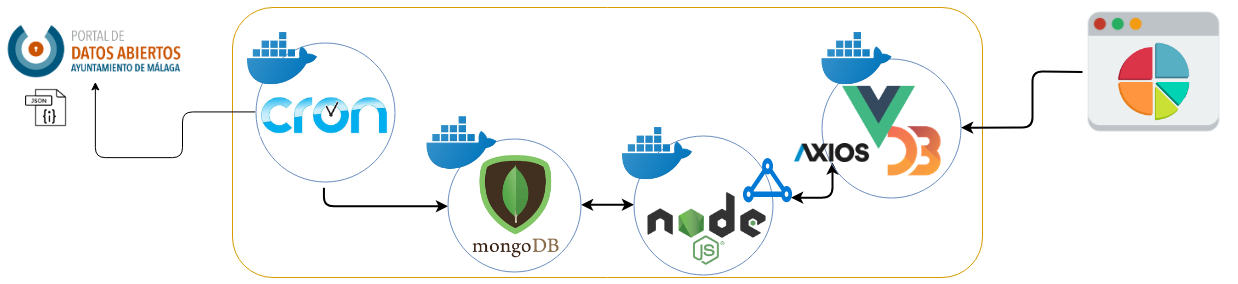
\includegraphics[width=12cm]{aireGuruArquitecture}
    \caption{Arquitecture Aire Guru}
\end{figure}

The data to the users through a web interface. \\

\begin{figure}[ht]
    \centering
    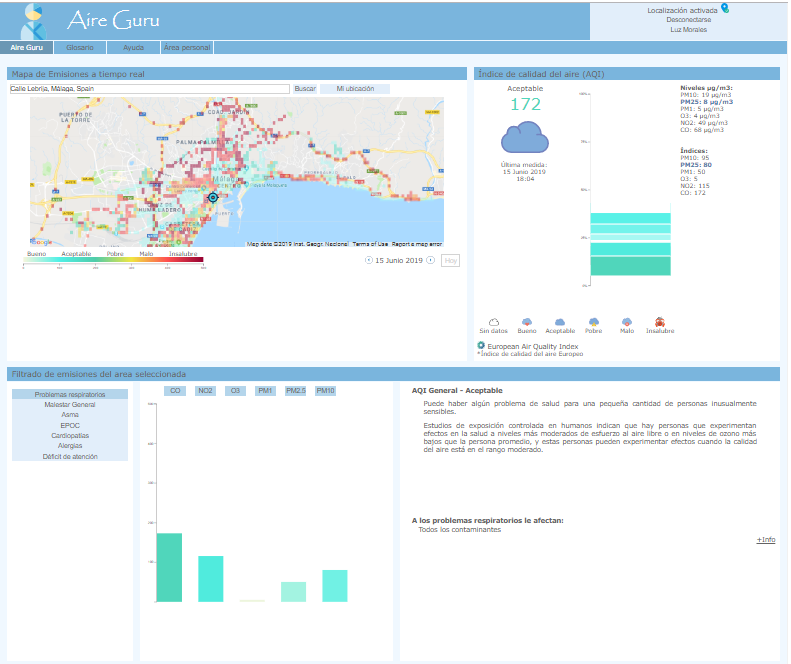
\includegraphics[width=9cm]{aireGuru}
    \caption{Aire Guru. Web Interface}
\end{figure}

To enable access by the majority of the population, Aire Guru is available at the web addresses https://www.aire.guru and https://www.airquality.guru.
We use SSL that guarantees the encryption of data through the network and ensure the user has access to it since, as more and more browsers try to protect 
users by only showing pages that use a secure method.

As we commented previously, all users can see the basic information without having to provide any data or identify themselves, without the need to
perform downloads or installations. Today, almost everyone is familiar with web browsing and if we do not force the user to realize extra taks, as 
requiring them to sign in or install extra software, the probability the user uses our platform will be higher. 

\newpage
\elsparagraph{Evaluation}  
\begin{itemize}
\done The data necessary for our model has been extracted from the raw data.
\done Infrastructure. Aire Guru implements all the necessary architecture of storage, processing and visualization so that the user only has to consult
the data.
\done It automates the processes of data collection and the necessary calculations to show the information to the user.
\done It offers users a free web page, and facilitates the users direct access to information.
\end{itemize}

